%%%%%%%%%%%%%%%%%%%%%%%%%%%%%%%%%%%%%%%%%
% Stylish Article
% LaTeX Template
% Version 2.1 (1/10/15)
%
% This template has been downloaded from:
% http://www.LaTeXTemplates.com
%
% Original author:
% Mathias Legrand (legrand.mathias@gmail.com) 
% With extensive modifications by:
% Vel (vel@latextemplates.com)
% Final ACS by:
% Juan Barbosa
% License:
% CC BY-NC-SA 3.0 (http://creativecommons.org/licenses/by-nc-sa/3.0/)
%
%%%%%%%%%%%%%%%%%%%%%%%%%%%%%%%%%%%%%%%%%
\documentclass[fleqn,11pt]{SelfArx}
%\usepackage[superscript]{cite}
\usepackage{wrapfig}
\usepackage{rotating}
\usepackage{subcaption}
\usepackage[numbers, super]{natbib}
%----------------------------------------------------------------------------------------
%	ARTICLE INFORMATION
%----------------------------------------------------------------------------------------

\JournalInfo{Laboratorio Org\'anica 3, No. 2, 15/09/2017} % Journal information
\Archive{ }

\PaperTitle{Reacci\'on de McMurry} %
%\Keywords{Keyword1 --- Keyword2 --- Keyword3} % Keywords - if you don't want any simply remove all the text between the curly brackets
%\newcommand{\keywordname}{Keywords} % Defines the keywords heading name

%----------------------------------------------------------------------------------------
%	ABSTRACT
%----------------------------------------------------------------------------------------

\Abstract{
\begin{wrapfigure}{r}{0.4\textwidth}
	\centering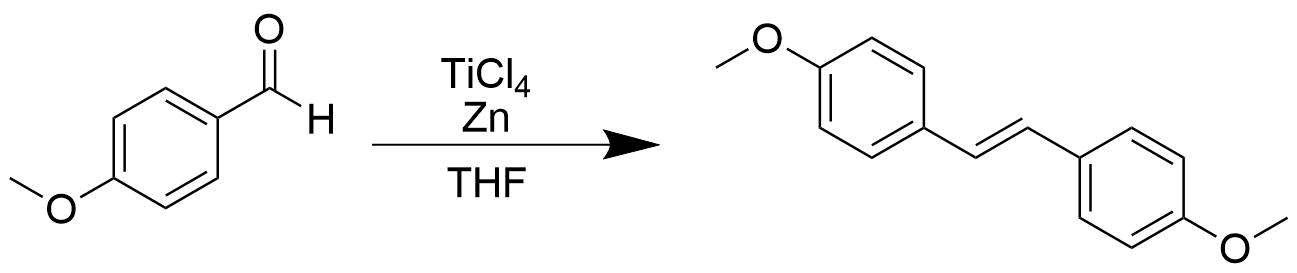
\includegraphics[width=\linewidth]{structures/Reaction.png}
\end{wrapfigure}

La preparaci\'on del (\textit{E})-1,2-bis(4-metoxifenil)eteno se llev\'o a cabo usando 4-metoxibenzaldehido, cloruro de titanio (IV) y zinc como agente reductor, en una reacci\'on de McMurry, usando tetrahidrofurano como disolvente. La reacci\'on tuvo una duraci\'on de 19 horas y un rendimiento superior al 8 \%. La caracterizaci\'on del producto se llev\'o a cabo usando $^1$HRMN y $^{13}$CRMN. 
}

%----------------------------------------------------------------------------------------

\begin{document}

\flushbottom % Makes all text pages the same height

\maketitle % Print the title and abstract box

%\tableofcontents % Print the contents section

\thispagestyle{empty} % Removes page numbering from the first page
\renewcommand{\tablename}{Tabla} 
%----------------------------------------------------------------------------------------
%	ARTICLE CONTENTS
%----------------------------------------------------------------------------------------

\section*{Introducci\'on} % The \section*{} command stops section numbering
%------------------------------------------------

La reacci\'on de McMurry fue publicada en 1974, por John E. McMurry. Si bien var\'ios art\'iculos fueron publicados en la d\'ecada de los 70 \cite{Mukaiyama1973, Mukaiyama1974} sobre reacciones de acoplamiento reductivo de carbonilos a alquenos usando esp\'ecies de titanio con bajo estado de oxidaci\'on, fue McMurry el que hizo un estudio detallado de los alcances de la reacci\'on \cite{Wang2010}.

La reacci\'on de McMurry es muy usada para la formaci\'on de alquenos a partir de aldeh\'idos, siendo una ventaja importante la posibilidad de realizar acoplamientos intra e intermoleculares de aldeh\'idos y cetonas en macrociclos \cite{Wang2010, Villiers1997}. La reacci\'on tiene lugar con varias esp\'ecies de titanio, con estados de oxidaci\'on $+2$ y $+3$ producidos \textit{in situ}, con un agente reductor. Una gran cantidad de agentes reductores han sido usados en la reacci\'on de McMurry, ejemplos de estos son: \ce{Mg}, \ce{Zn}, \ce{LiAlH4}, \ce{LiBH4}, \ce{LiH}, \ce{CaH2} \cite{Wang2010}.
\begin{scheme}[h]
	\centering
	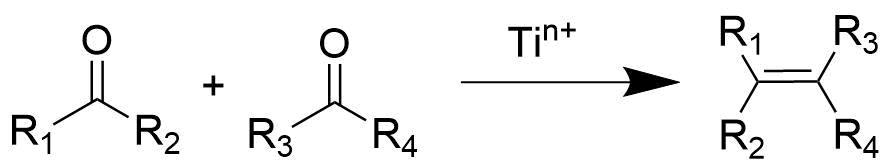
\includegraphics[width=0.9\linewidth]{structures/generalreaction.png}
	\caption{Reacci\'on general de McMurry. El estado de oxidaci\'on del titanio es $1\leq n\leq3$. \ce{R1, R3}: alquil o aril, \ce{R2, R4}: H, alquil o aril \cite{Wang2010}.}
\end{scheme}

Los alquenos producidos por este m\'etodo suelen ser mayoritariamente \textit{trans}, sin embargo existen casos donde se da el \textit{cis}. El control de la estereoqu\'imica en la reacci\'on de McMurry es limitado por el tama\~no de las mol\'eculas reactantes \cite{Rele2001, Wang2010}.
\pagebreak

\begin{scheme}[h]
	\centering
	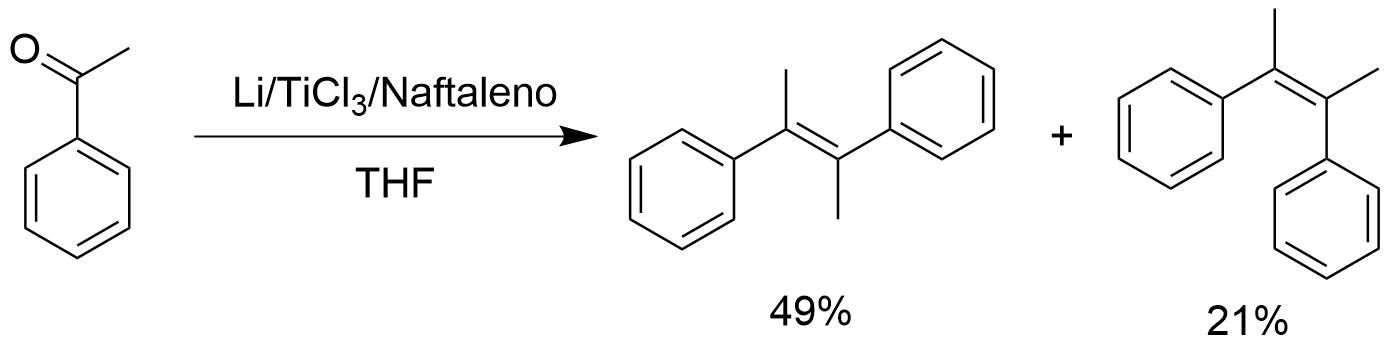
\includegraphics[width=0.8\linewidth]{structures/EZselectivity.png}
	\caption{La selectividad de la reacci\'on est\'a dada por el tamaño de la mol\'ecula \cite{Rele2001, Wang2010}.}
\end{scheme}

Por otro lado la reacci\'on funciona mejor en los casos donde el acoplamiento se da entre compuestos arom\'aticos \cite{Wang2010}, sin embargo tambi\'en ocurre con menor frecuencia en compuestos alif\'aticos \cite{Rele2001}. Para que la reacci\'on se lleve acabo son necesarias altas temperaturas y tiempos prolongados para la desoxigenaci\'on de la mol\'ecula \cite{Wang2010, Villiers1997}.
\begin{figure*}[ht]
	\centering
	\begin{subfigure}[t]{0.49\linewidth}
		\centering
		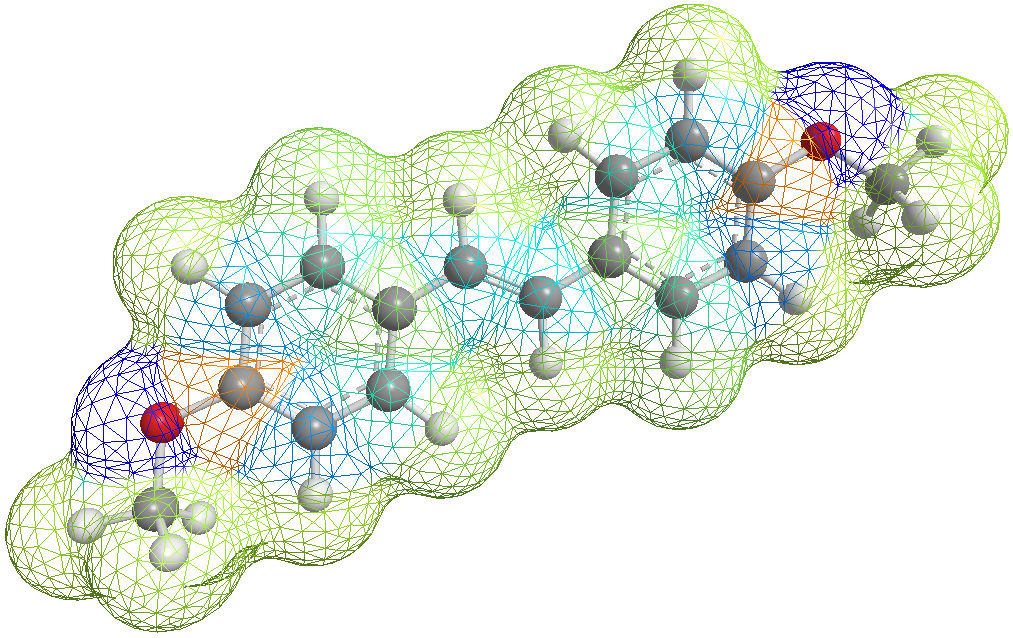
\includegraphics[width=0.9\linewidth]{structures/productE.png}
		\caption{(\textit{E})-1,2-bis(4-metoxifenil)eteno, $E=12.1013$ kcal/mol.}
	\end{subfigure}
	\begin{subfigure}[t]{0.49\linewidth}
		\centering
		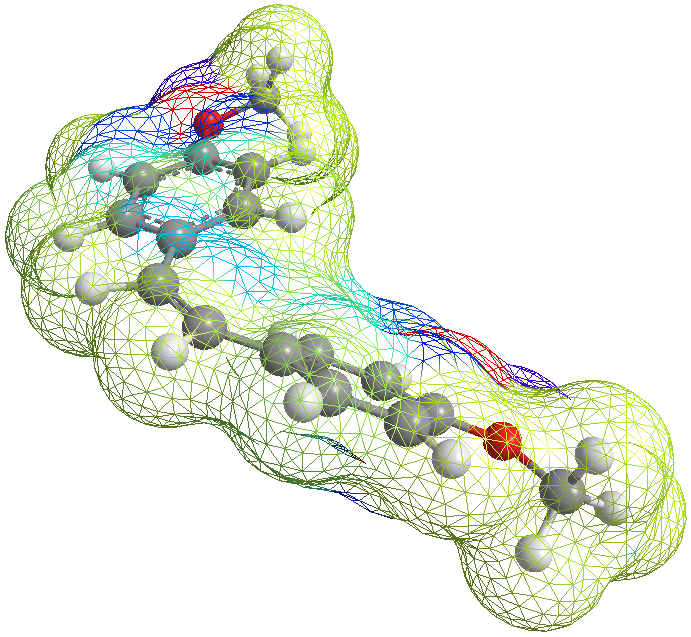
\includegraphics[width=0.7\linewidth]{structures/productZ.png}
		\caption{(\textit{Z})-1,2-bis(4-metoxifenil)eteno, $E=23.4982$ kcal/mol.}
	\end{subfigure}
	\caption{Estereoqu\'imica de los posibles productos de la reacci\'on de McMurry. El color viene de la densidad de carga: azul para los valores m\'inimos y rojo para valores m\'aximos. La energ\'ia es calculada usando un algoritmo de segunda generaci\'on de \textit{Mining-Minima} (MM2)\cite{Huang2012}.}
	\label{fig: both}
\end{figure*}

\begin{scheme}[h]
	\centering
	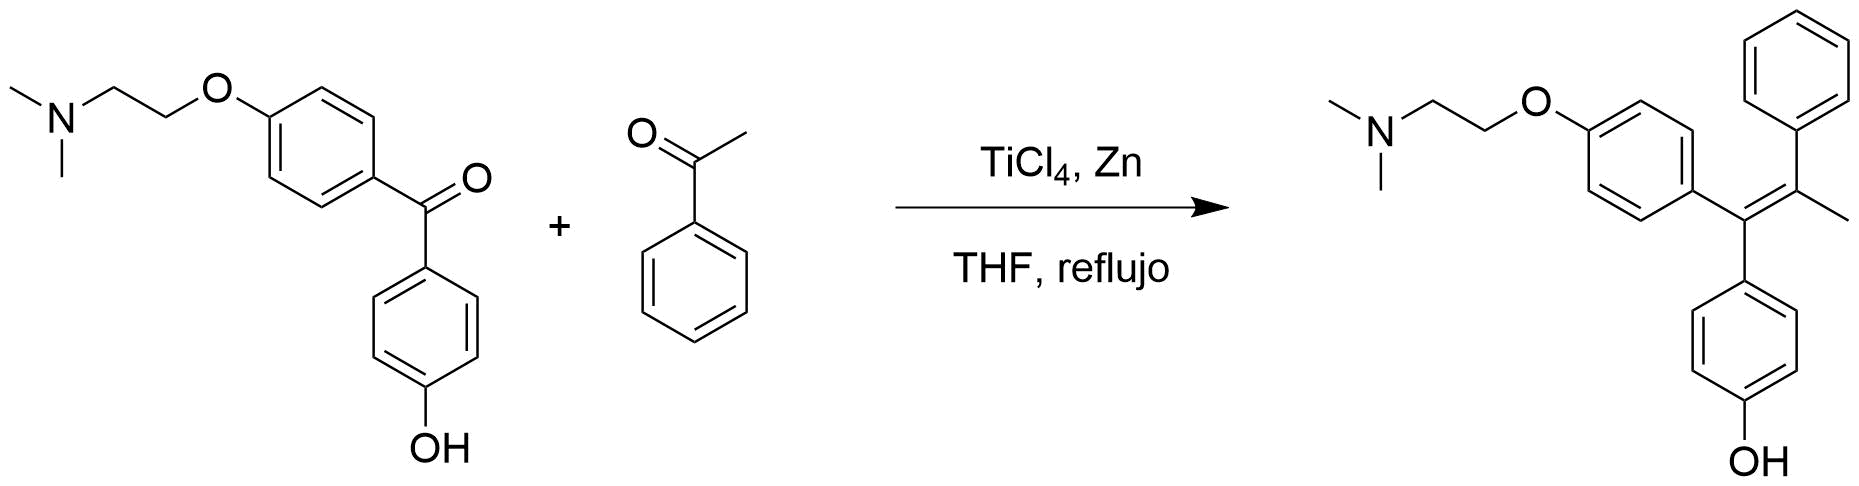
\includegraphics[width=0.9\linewidth]{structures/Tamoxifeno.png}
	\caption{An\'alogo al Tamoxifeno usando una reacci\'on de McMurry \cite{Zheng2007}.}
	\label{sch: tamoxifeno}
\end{scheme}
El Tamoxifeno es un medicamento conocido por su actividad con el modulador selectivo de los receptores estrog\'enicos, un compuesto que inhibe la acci\'on de los estr\'ogenos en ciertos tejidos, mientras la simula en otros. Ampliamente usado para el tratamiento y prevenci\'on del cancer de mama, este medicamento cuenta con algunos an\'alogos en donde se modifican los sustituyentes, un ejemplo de estos se muestra como producto en el \autoref{sch: tamoxifeno}, el cual se obtiene usando una reacci\'on de McMurry en la etapa final de la s\'intesis, siendo el \textit{Z} el \'unico is\'omero formado \cite{Zheng2007}.

\section{Resultados y Discusi\'on}
La masa del producto obtenido es de 0.1222 g, la relaci\'on estequeom\'etrica entre el \textit{p}-metoxibenzaldeh\'ido con el (\textit{E})-1,2-bis(4-metoxifenil)eteno es 2:1, lo anterior junto con la cantidad de \textit{p}-metoxibenzaldeh\'ido usado implica un 20.3 \% de recuperaci\'on. Sin embargo lo anterior supone dos cosas: tanto que el reactivo de partida como el producto obtenido se encuentran puros. Ambas de estas suposiciones se presumen falsas, la primera porque el aldeh\'ido no fue destilado, por lo cual es posible que existan trazas del \'acido en el mismo. Lo anterior no se puede confirmar con los espectros de RMN porque el \'acido pudo haber sido arrastrado en la soluci\'on acuosa al momento de realizar la extracci\'on l\'iquido l\'iquido. Por el otro lado el espectro de RMN muestra v\'arias señales adicionales a las de la muestra, lo cual de entrada implica que no es un producto puro. La cuantificaci\'on de los contaminantes tiene un efecto negativo sobre el porcentaje de recuperaci\'on, es decir lo disminuye. Por el contrario la contaminaci\'on en el reactivo de partida tiene un efecto positivo sobre el porcentaje, dado que los dos efectos son contarios, no es posible acotar el porcentaje de recuperaci\'on, sin determinar la magnitud de uno de ellos.

La cuantificaci\'on de los contaminantes en el producto se realiza usando las siquientes ecuaciones:
\begin{equation}
	R_{(p, i)} = \left(\dfrac{n_H^{(p)}}{I_H^{(p)}}\right)\left(\dfrac{I_H^{(i)}}{n_H^{(i)}}\right)
\end{equation}

\pagebreak
Donde $R_{(p, i)}$ es la relaci\'on producto impureza, esto es el n\'umero de mol\'eculas de una impureza por cada mol\'ecula de producto. $n^{(p)}$ corresponde con el n\'umero de hidr\'ogenos integrados en el producto, $I^{(p)}$ el valor de la integral en el $^1$HRMN.

\begin{equation}
	C_{rel} = \dfrac{R_{(p, i)}PM_{i}}{\sum\limits_{j=1}^N R_{(p, j)}PM_{j}}
\end{equation}

Donde $C_{rel}$ es la cantidad relativa en masa del compuesto $i$ en la muestra, $PM_j$ es el peso molecular del compuesto $j$, y $N$ el n\'umero de compuestos identificados.
\begin{table}[h]
	\centering
	\caption{Cuantificaci\'on de los contaminantes. La señal usada para el THF est\'a en 3.75 ppm \cite{Fulmer2010}, y para el \ce{C16H18O4} la señal de los metoxis en 3.78 ppm.}
	\begin{tabular}{ccccc}
		\hline
		\textbf{Compuesto} & $n_H$ & $I_H$ & $R_{(p, j)}PM_j$ & $C_{rel}$ \\
		\hline
		\ce{THF} & 2 & 7.98 & 276.49 & 0.46 \\
		\ce{C16H18O4} & 6 & 0.29 & 79.96 & 0.13 \\
		\hline
	\end{tabular}
	\label{tb: composicion}
\end{table}

La concentraci\'on del compuesto de inter\'es en la muestra es de 41 \%. Por lo cual considerando el efecto de las impurezas se calcula un porcentaje de recuperaci\'on del 8 \%, sin embargo como se discuti\'o anteriormente al considerar impurezas en el reactivo de partida el porcentaje de recuperaci\'on sera mayor o igual al 8 \%. Como se observa en la \autoref{tb: composicion} existe una gran cantidad de THF en la muestra, por esta raz\'on se recomienda cambiar el disolvente usado en la extraci\'on l\'iquido l\'iquido de menor polaridad.
\begin{scheme}[h]
	\centering
	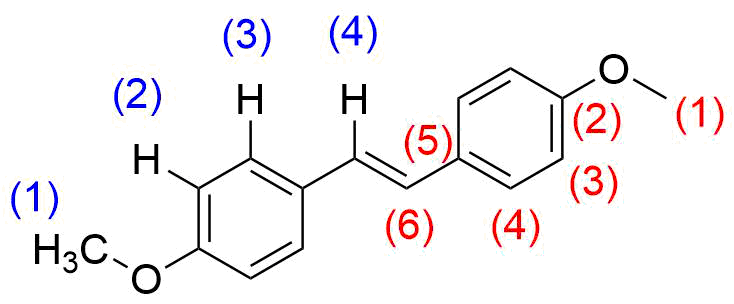
\includegraphics[width=0.7\linewidth]{structures/RMN.png}
	\caption{Asignaci\'on de señales de RMN, en azul se enumeran los protones y en rojo los carbonos.}
\end{scheme}

Para la identificaci\'on del producto se tiene en cuenta la simetr\'ia de la mol\'ecula, en la muestra existen cuatro ambientes químicos distintos para los protones. El ambiente m\'as protegido corresponde con el del grupo metoxi \textbf{(1)}, para el cual se observa una señal singlete que integra para 6 hidr\'ogenos a 3.79 ppm. A campo m\'as bajo, en 6.83 ppm, se encuentra la señal de los hidr\'ogenos vin\'ilicos, estos est\'an m\'as desprotegidos que un enlace doble com\'un por la cercan\'ia a los grupos fenilo \textbf{(4)}. Tanto el grupo vinilo como metoxi constituyen grupos activantes, sin embargo el ox\'igeno introduce m\'as carga al anillo en las posiciones \textit{orto} y \textit{para} al metoxi, por esta raz\'on los protones en las posiciones \textbf{(2)} se encuentran a 6.95 ppm, mientras que la señal \textbf{(3)} aparece en 7.11, ambas señales corresponden a dobletes en la regi\'on arom\'atica y cada una integra para cuatro hidr\'ogenos. 

En el caso de los carbonos existen seis ambientes qu\'imicos, el m\'as protegido corresponde con el carbono del metoxi (55.27 ppm)\textbf{(1)}, seguido de los carbonos \textit{para} al metoxi (113.94 ppm)\textbf{(3)}, los carbonos vin\'ilicos siguen a campo m\'as bajo (128.47 ppm)\textbf{(6)}, desp\'ues se encuentras las señales de los carbonos \textit{meta} al metoxi junto con el carbono cuaternario del enlace vinil-benceno (130.16 ppm)\textbf{(4,5)}. El carbono m\'as deprotegido corresponde con el carbono (158.98 ppm)\textbf{(2)} al cual la electronegatividad del ox\'igeno le reduce la densidad de carga. Las señales de RMN corresponden con las reportadas en la literatura \cite{Zhong2016}. 

El experimento de DEPT-135 confirma la identidad de los carbonos, dado que los carbonos \textbf{(5)} y \textbf{(2)} no son visibles, el resto aparecen con el mismo desplazamiento y con intensidades positivas, propias de carbonos primarios y terciarios.

Respecto a la reacci\'on, la misma se lleva a cabo en tetrahidrofurano por dos razones: la primera es que el cloruro de titanio (IV) es soluble en THF, y por otro lado este disolvente no se reduce por las condiciones de la reacci\'on \cite{richards2001}. El primer paso de la reacci\'on corresponde con la reducci\'on del titanio (IV) en presencia de zinc (\autoref{eq: reduccion}), lo cual se realiza en reflujo por una hora.
\begin{equation}\label{eq: reduccion}
	\ce{TiCl4 + Zn ->[\Delta] TiCl2 + ZnCl2}
\end{equation}

La segunda parte de la reacci\'on mecan\'isticamente se divide en dos etapas. La primera es la formaci\'on del pinacol seguida de la desoxigenaci\'on del mismo. Aquí se discuten dos posibles mecanismos para la reacci\'on de acoplamiento. 

En el \autoref{sch: primer} se muestra el primer mecanismo propuesto, una vez se adiciona el \textit{p}-metoxibenzaldehido al medio de reacci\'on un electr\'on de valencia del titanio ataca al ox\'igeno generando a su vez un radical sobre el carbono carbon\'ilico \textbf{(a)}. Posteriormente el radical de titanio ataca de forma an\'aloga a otra mol\'ecula de aldeh\'ido \textbf{(b)}. Luego tiene lugar la ciclaci\'on \textbf{(c)}, en este punto dos posibles intermediarios se pueden formar dependiendo de la orientaci\'on de los ciclos.

\begin{scheme}[h]
	\centering
	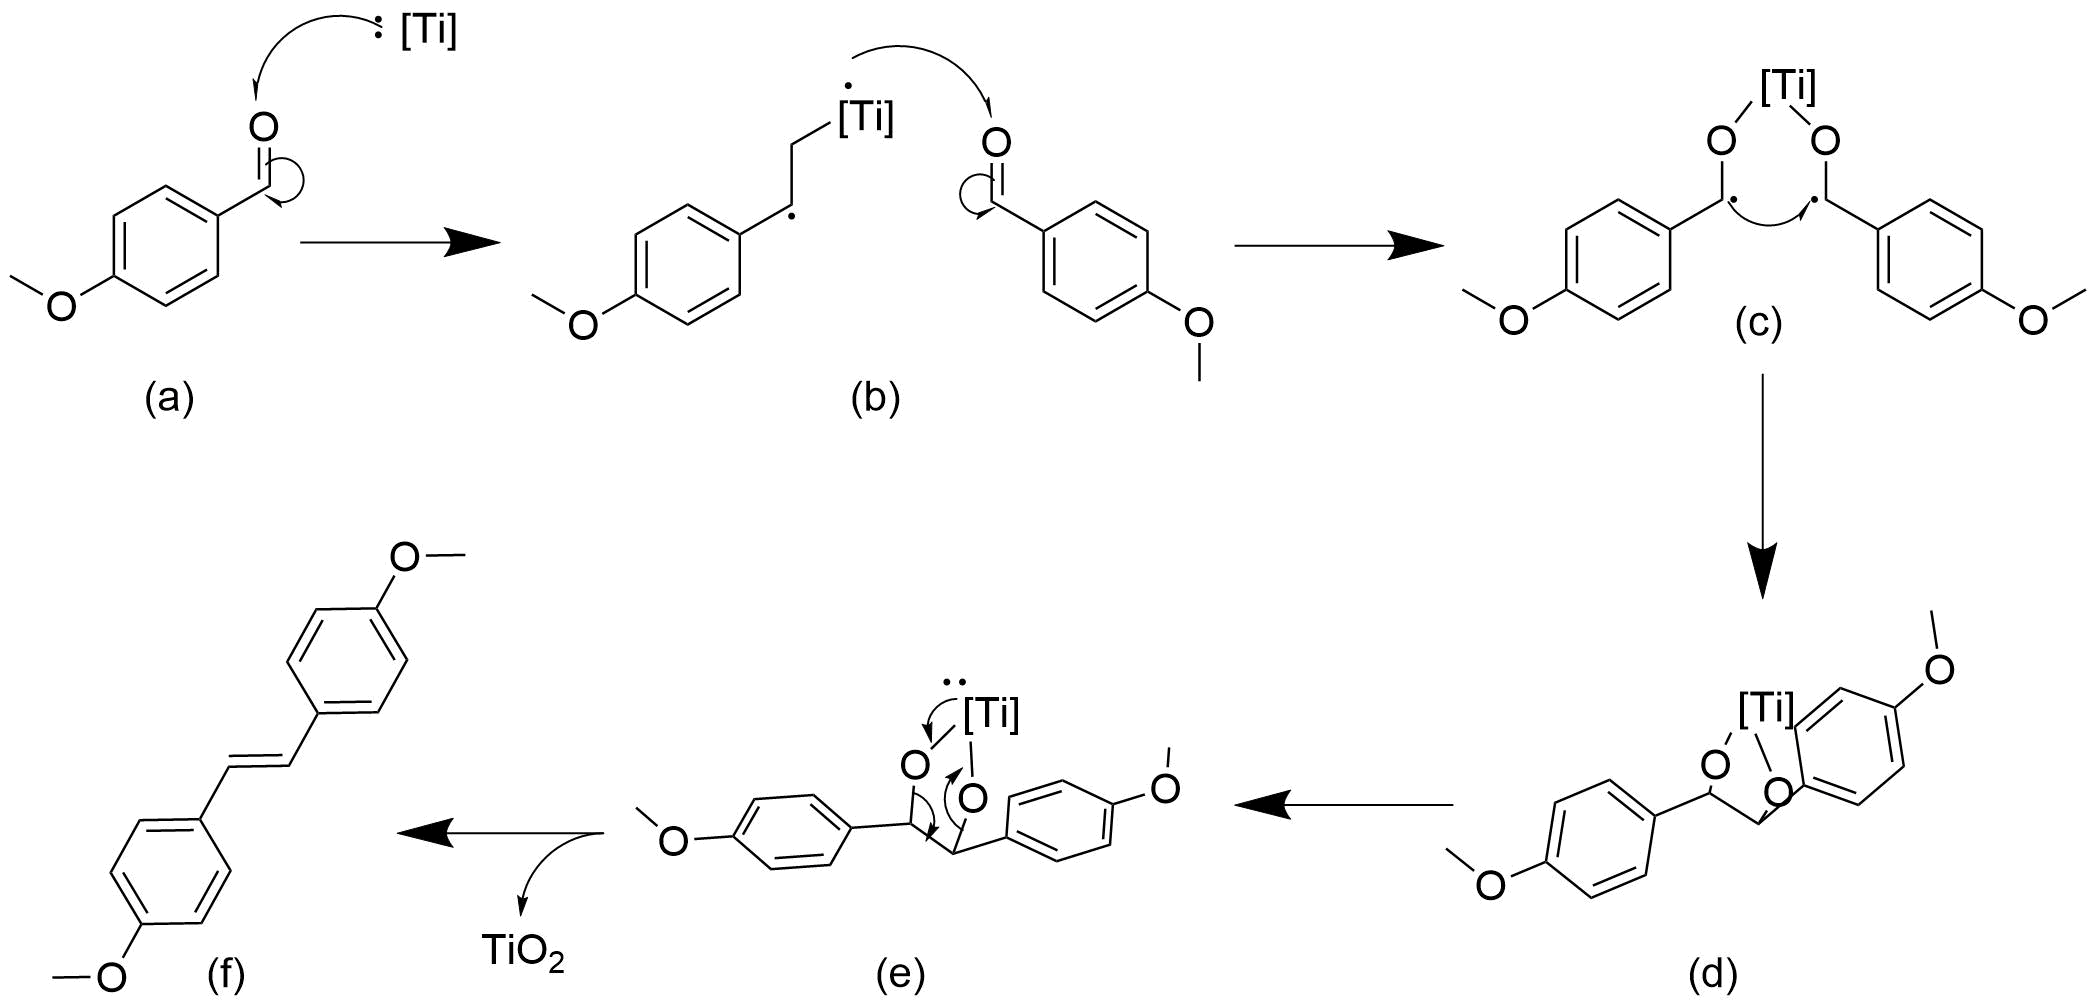
\includegraphics[width = \linewidth]{structures/mechanism.png}
	\caption{Primer mecanismo de reacci\'on propuesto.}
	\label{sch: primer}
\end{scheme}

Teniendo en cuenta el volumen de los ciclos y las interacciones desfavorables que se tienen si ambos se encuentran muy cerca, la ciclaci\'on se da a manera de puente (\textit{R, R}), esto porque la energ\'ia total de la mol\'ecula con estereoqu\'imica (\textit{R, R}) es cerca de la mitad de la de estereoqu\'imica (\textit{R, S}) (\autoref{fig: both}). La informaci\'on de la energ\'ia es particularmente útil teniendo en cuenta que los estados de transici\'on y los productos de menor energ\'ia est\'an favorecidos. La formaci\'on de un pinacol \textbf{(d)}, da paso a la desoxigenaci\'on de la mol\'ecula, generando el producto de estereoqu\'imica \textit{E} \cite{richards2001}. Cabe mencionar que seg\'un este mecanismo, si el ciclo formado en el paso \textbf{(c)} tiene la estereoqu\'imica (\textit{R, S}) el producto final ser\'a el \textit{Z} (energ\'eticamente desfavorable).
\begin{scheme}[h]
	\centering
	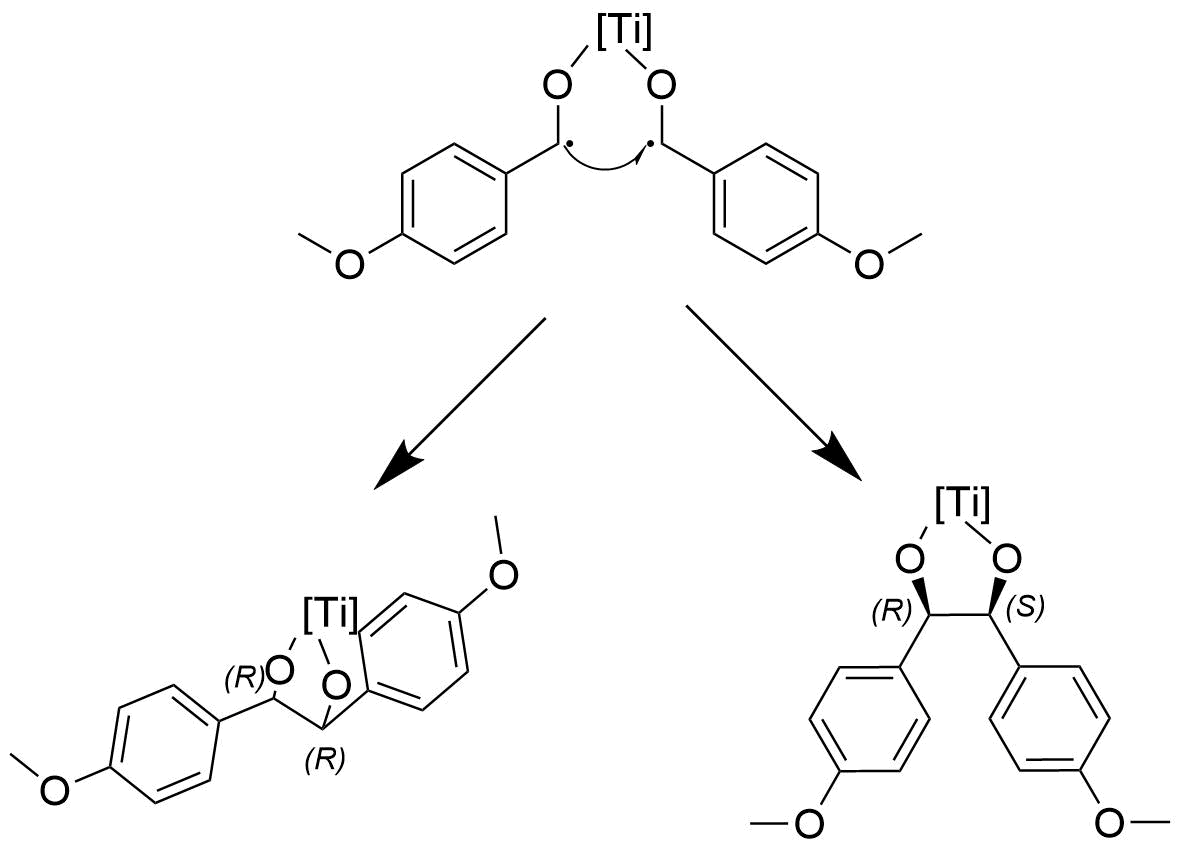
\includegraphics[width = 0.8\linewidth]{structures/EZdetermined.png}
	\caption{Posibles formas en las que tiene lugar la ciclaci\'on.}
	\label{sch: EZ}
\end{scheme}

El segundo mecanismo propuesto se presenta en el \autoref{sch: segundo}, e involucra una relaci\'on estequiom\'etrica titanio-producto (4:1). En este caso el ataque del titanio se da por aparte en dos mol\'eculas de \textit{p}-benzaldeh\'ido \textbf{(g)}. Posteriormente tiene lugar el acoplamiento con los radicales, en este paso tambi\'en es posible que se formen los estereois\'omeros (\textit{R, R}) \'o (\textit{R, S}) an\'alogo al \autoref{sch: EZ}. Posteriormente tiene lugar la desoxigenaci\'on con la formaci\'on de un nuevo enlace titanio \'oxigeno sobre los dos ox\'igenos de la mol\'ecula, y la formaci\'on de un enlace $\pi$ carbono-carbono \textbf{(j)} \cite{Wang2010}.
\begin{scheme}[h]
	\centering
	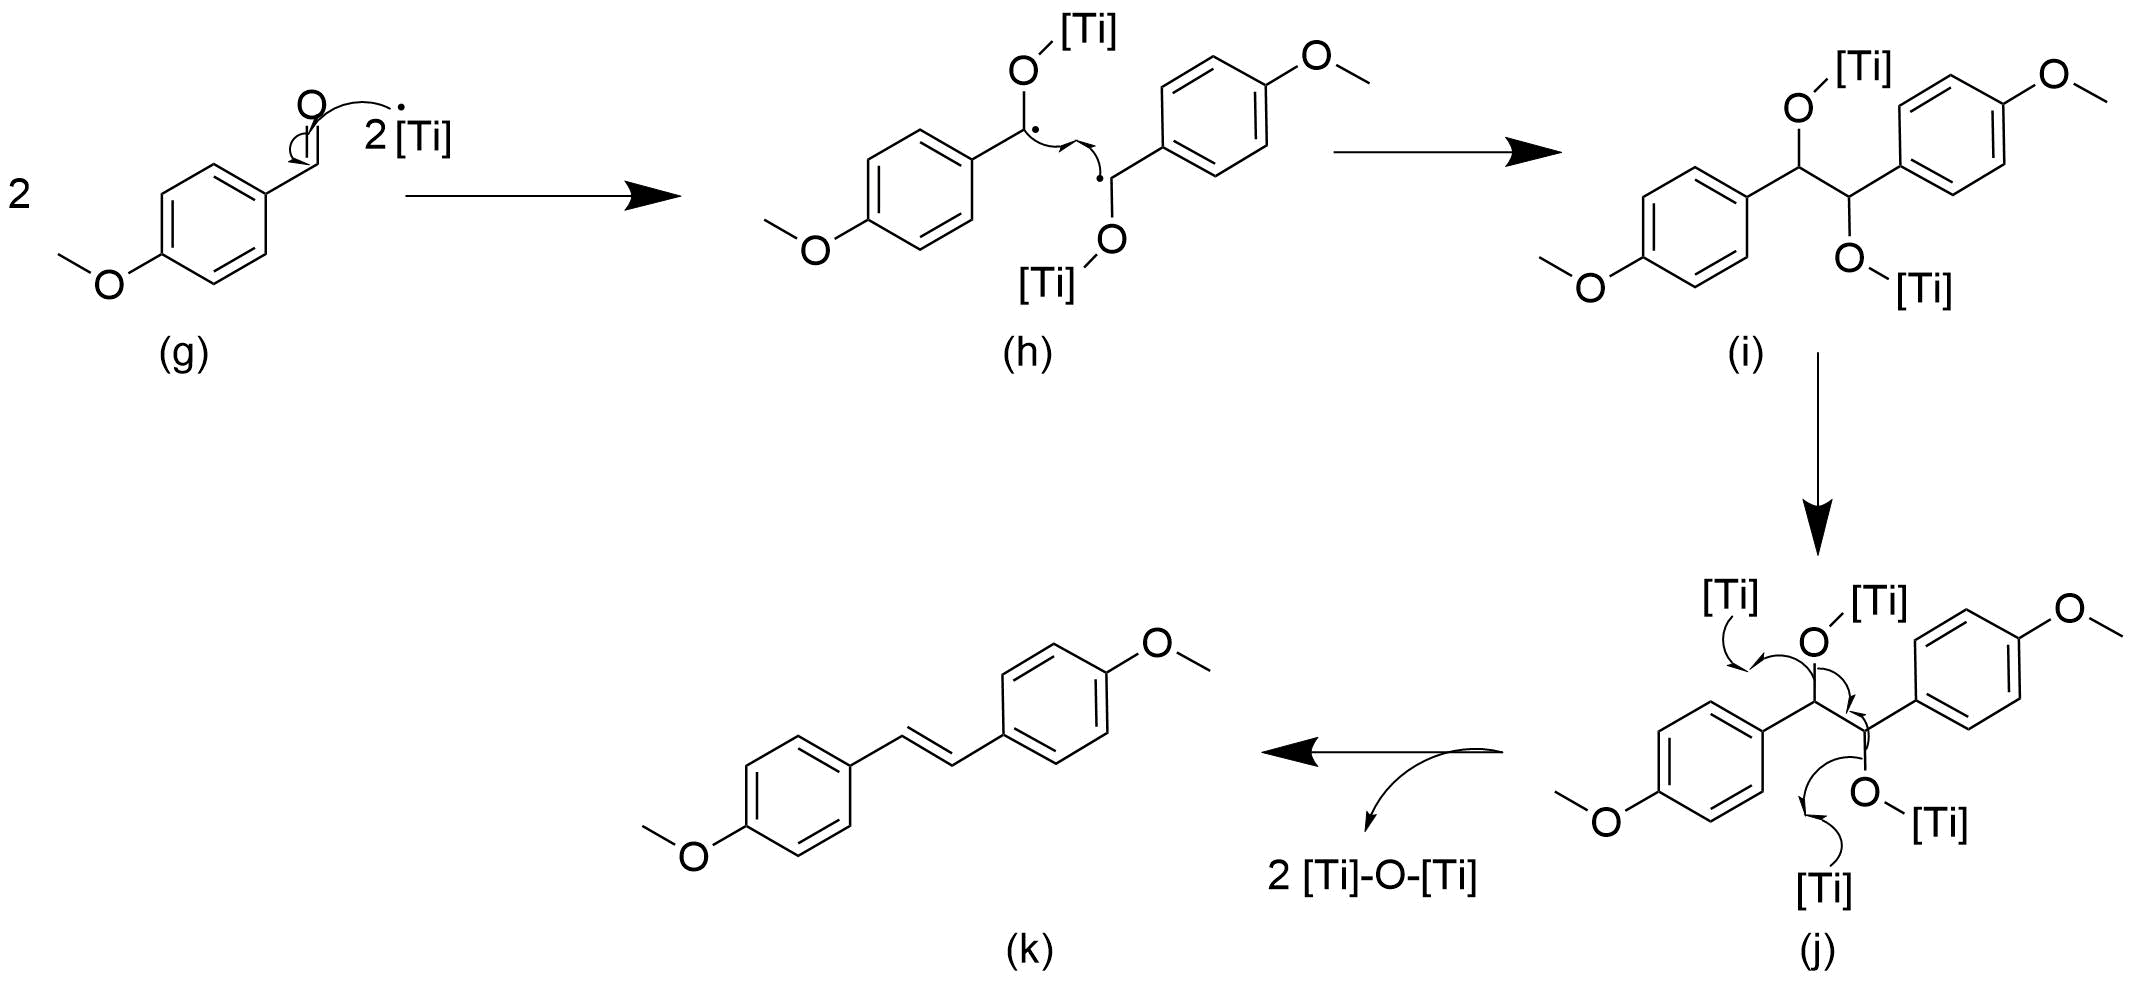
\includegraphics[width = \linewidth]{structures/mechanism2.png}
	\caption{Segundo mecanismo de reacci\'on propuesto \cite{Wang2010}.}
	\label{sch: segundo}
\end{scheme}

Es posible que ambos mecanismos ocurran en el medio de reacci\'on, en funci\'on de las esp\'ecies de titanio disponibles. Para el caso del titanio (II) o el titanio (0) el mecanismo preferente ser\'a el del \autoref{sch: primer}, mientras que el titanio (III) tender\'a a seguir el mecanismo del \autoref{sch: segundo}. En el caso del producto \autoref{sch: titanio1} el mismo puede ser reducido por el Zn presente en el medio para formar cloruro de zinc (II) y \'oxido de titanio (IV).
\begin{scheme}[h]
	\centering
	\scriptsize
	\begin{subfigure}[t]{0.49\linewidth}
		\centering
		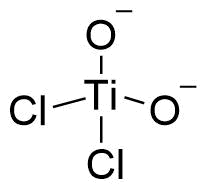
\includegraphics[width=0.4\linewidth]{structures/titanium1.png}
		\caption{Producto del Ti (II).}
		\label{sch: titanio1}
	\end{subfigure}
	\begin{subfigure}[t]{0.3\linewidth}
		\centering
		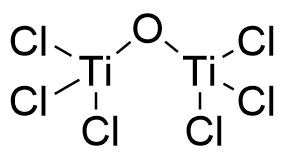
\includegraphics[width=0.9\linewidth]{structures/titanium2.png}
		\caption{Producto del Ti (III).}
		\label{sch: titanio2}
	\end{subfigure}
	\caption{Complejos asociados a los mecanismos propuestos.}
\end{scheme}

\pagebreak
Ambos mecanismos propuestos son susceptibles al efecto del agua en la reacci\'on, tanto los compuestos \textbf{(d)} como \textbf{(i)} en contacto con agua dar\'an lugar a la formaci\'on del diol, compuesto que se muestra en el \autoref{sch: diol}.
\begin{scheme}[h]
	\centering
	\scriptsize
	\begin{subfigure}[t]{0.49\linewidth}
		\centering
		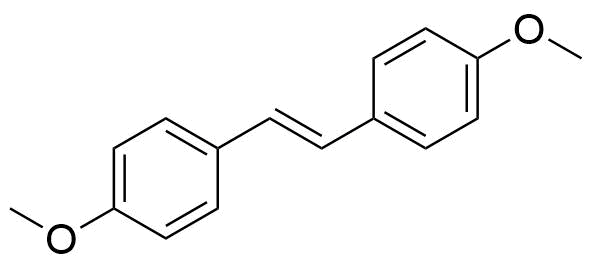
\includegraphics[width=0.9\linewidth]{structures/product.png}
		\caption{(\textit{E})-1,2-bis(4-metoxifenil)eteno}
		\label{sch: producto}
	\end{subfigure}
	\begin{subfigure}[t]{0.49\linewidth}
		\centering
		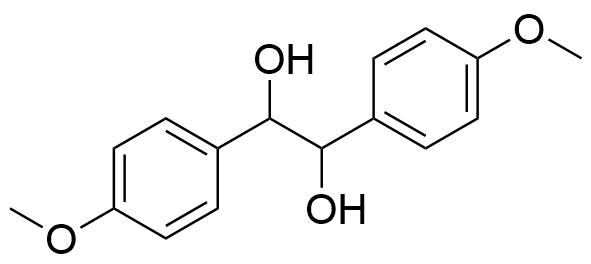
\includegraphics[width=0.9\linewidth]{structures/product2.png}
		\caption{1,2-bis(4-metoxifenil)etano-1,2-diol}
		\label{sch: diol}
	\end{subfigure}
	\caption{Productos de la reacci\'on.}
\end{scheme}

La presencia del compuesto di\'olico se confirma por t\'ecnicas espectrosc\'opicas, en donde se observan señales de hidr\'ogeno en 3.75 ppm, 4.79 ppm, y 7.26 ppm, señales que se encuentran reportadas para el diol en la literatura \cite{Uchiyama2004}. La informaci\'on anterior indica que el THF no se encontraba completamente seco al momento de realizar la reacci\'on, o bien existi\'o una fuga en la atm\'osfera de la reacci\'on.

La reacci\'on de McMurry est\'a relacionada con la reacci\'on de Barton-Kellogg en la cual se efect\'ua un acomplamiento entre un diazocompuesto y una tiocetona o tioaldeh\'ido, dando lugar a un alqueno. Tanto la tiocetona como el diazocompuesto pueden ser obtenidos a partir de aldeh\'idos y cetonas \cite{Barton1970, Kellogg1970, Wang2010}. Una ruta alterna para obtener el (\textit{E})-1,2-bis(4-metoxifenil)eteno usando la reacci\'on de Barton-Kellogg implica el tratamiento del $p$-metoxibenzaldeh\'ido con hidrazina para producir la hidrazona con posterior oxidaci\'on para conseguir el 1-(diazometil)-4-metoxibenzeno, adem\'as de la obtenci\'on del 4-metoxibenzotialdeh\'ido.

\begin{scheme}[h]
	\centering
	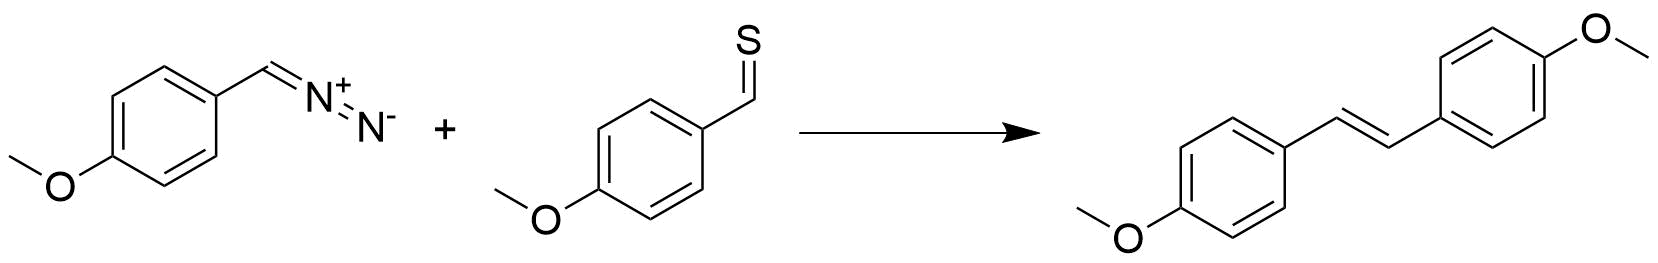
\includegraphics[width=\linewidth]{structures/Barton.png}
	\caption{Obtenci\'on del (\textit{E})-1,2-bis(4-metoxifenil)eteno usando la reacci\'on de Barton-Kellogg.}
\end{scheme}

\section{Conclusiones}
La preparaci\'on del (\textit{E})-1,2-bis(4-metoxifenil)eteno se realiz\'o usando una reacci\'on de McMurry, con un rendimiento superior o igual al 8 \%. El rendimiento no pudo ser establecido con exactitud dado que se desconoce la pureza del reactivo de partida. Se realizaron estudios computacionales para la determinaci\'on de la energ\'ia de los compuestos $E$ y $Z$ para as\'i sustentar la formaci\'on del compuesto $E$. Se recomienda el uso de un disolvente de menor polaridad para mejorar la extraci\'on l\'iquido l\'iquido y limitar el THF en el producto. Dos mecanismos de reacci\'on fueron propuestos junto con una preparaci\'on alternativa usando la reacci\'on de Barton-Kellogg, siendo esta considerablemente m\'as compleja dado que se requieren varios pasos para la obtenci\'on del producto.

\section{Secci\'on experimental}
50 mL de tetrahidrofurano previamente seco por 48 horas usando tamiz molecular, se agregan sobre un bal\'on de dos bocas junto con zinc (15.0 mmol) y cloruro de titanio (IV) (7.5 mmol). La soluci\'on se lleva a reflujo por 1 hora, pasada la cual se adiciona \textit{p}-metoxibenzaldeh\'ido (5.0 mmol). La reacci\'on se lleva a cabo a 55 $^\circ$C por 18 horas en atm\'osfera de nitrógeno. La reacci\'on es tratada en 50 mL de \'acido clorh\'idrico 1 M. Se realiza una filtraci\'on en celita y una extracci\'on l\'iquido l\'iquido con dos lavados de 15 mL de diclorometano. El extracto se baña en salmuera y se extrae el sobrenadante, el cual se seca usando sulfato de magnesio y se evapora el disolvente.

Una etapa de purificaci\'on se realizó usando una columna de s\'ilica y se eluy\'o el crudo usando una fase m\'ovil de acetato de etilo-pentano (4 : 6), se recolectaron las fracciones 3-6, las cuales se concentraron con la evaporaci\'on del disolvente.

\paragraph{4-metoxibenzaldehido:}
$^1$H NMR (400 MHz, \ce{CDCl3}) $\delta$ 7.11 (d, 4H), 6.95 (d, J = 32.8, 7.8 Hz, 4H), 6.83 (s, 2H), 3.81 (s, 6H).

$^{13}$C NMR (101 MHz, \ce{CDCl3}) $\delta$ 158.98 (s), 130.16 (s), 128.47 (s), 113.94 (s), 55.27 (s).

DEPT-135 (101 MHz, \ce{CDCl3}) $\delta$ 132.06 – 126.91 (m), 114.27 (s), 55.30 (s).
%----------------------------------------------------------------------------------------
%	REFERENCE LIST
%----------------------------------------------------------------------------------------
\phantomsection
\bibliography{informe}
\bibliographystyle{achemso}
%----------------------------------------------------------------------------------------
\newpage
\onecolumn
\section{Informaci\'on suplementaria}\label{sec: complementaria}
\rotatebox{90}
{
	\begin{minipage}{0.9\textheight}
		\centering
		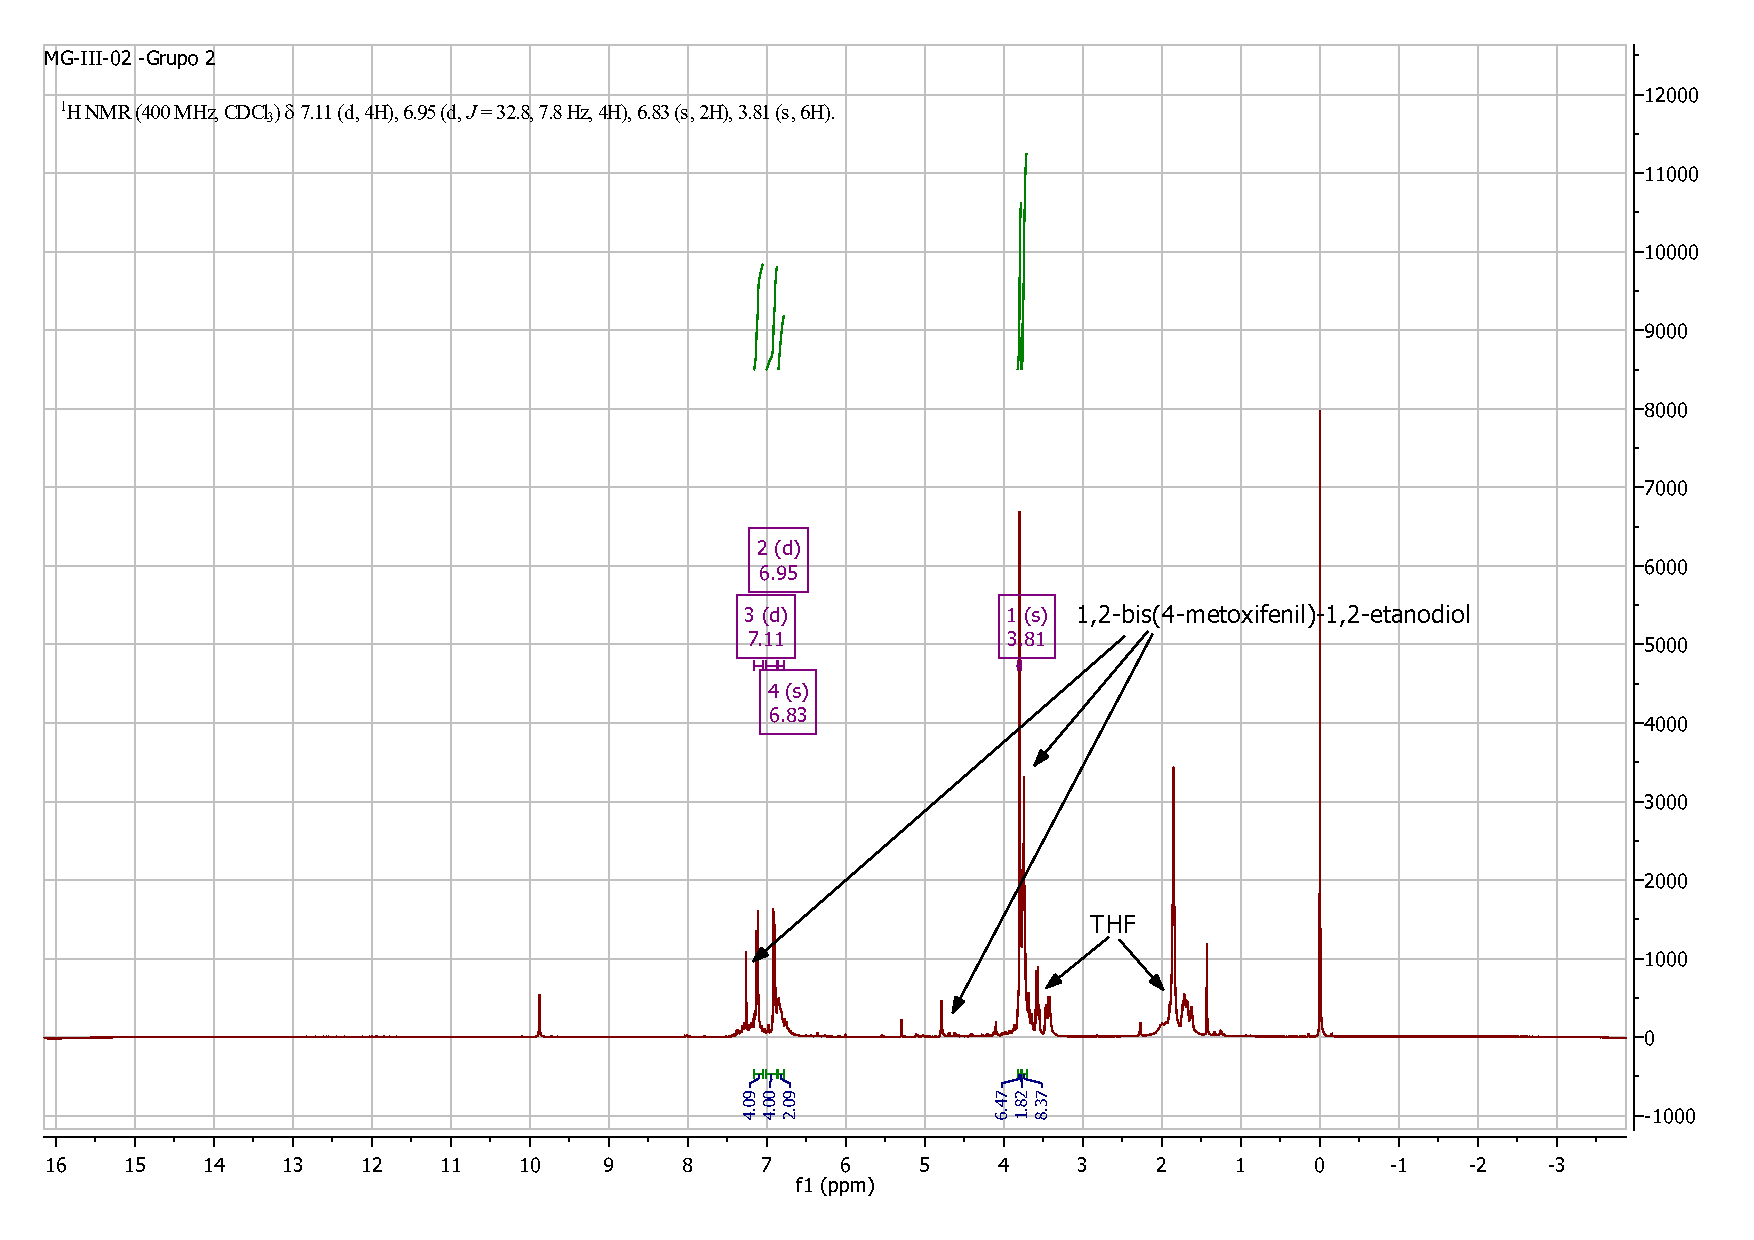
\includegraphics[height=0.7\textheight]{RMN/H.pdf}
		\captionof{figure}{$^{1}$HRMN del producto purificado.}
		\label{HHRM}
	\end{minipage}
}

\rotatebox{90}
{
	\begin{minipage}{\textheight}
		\centering
		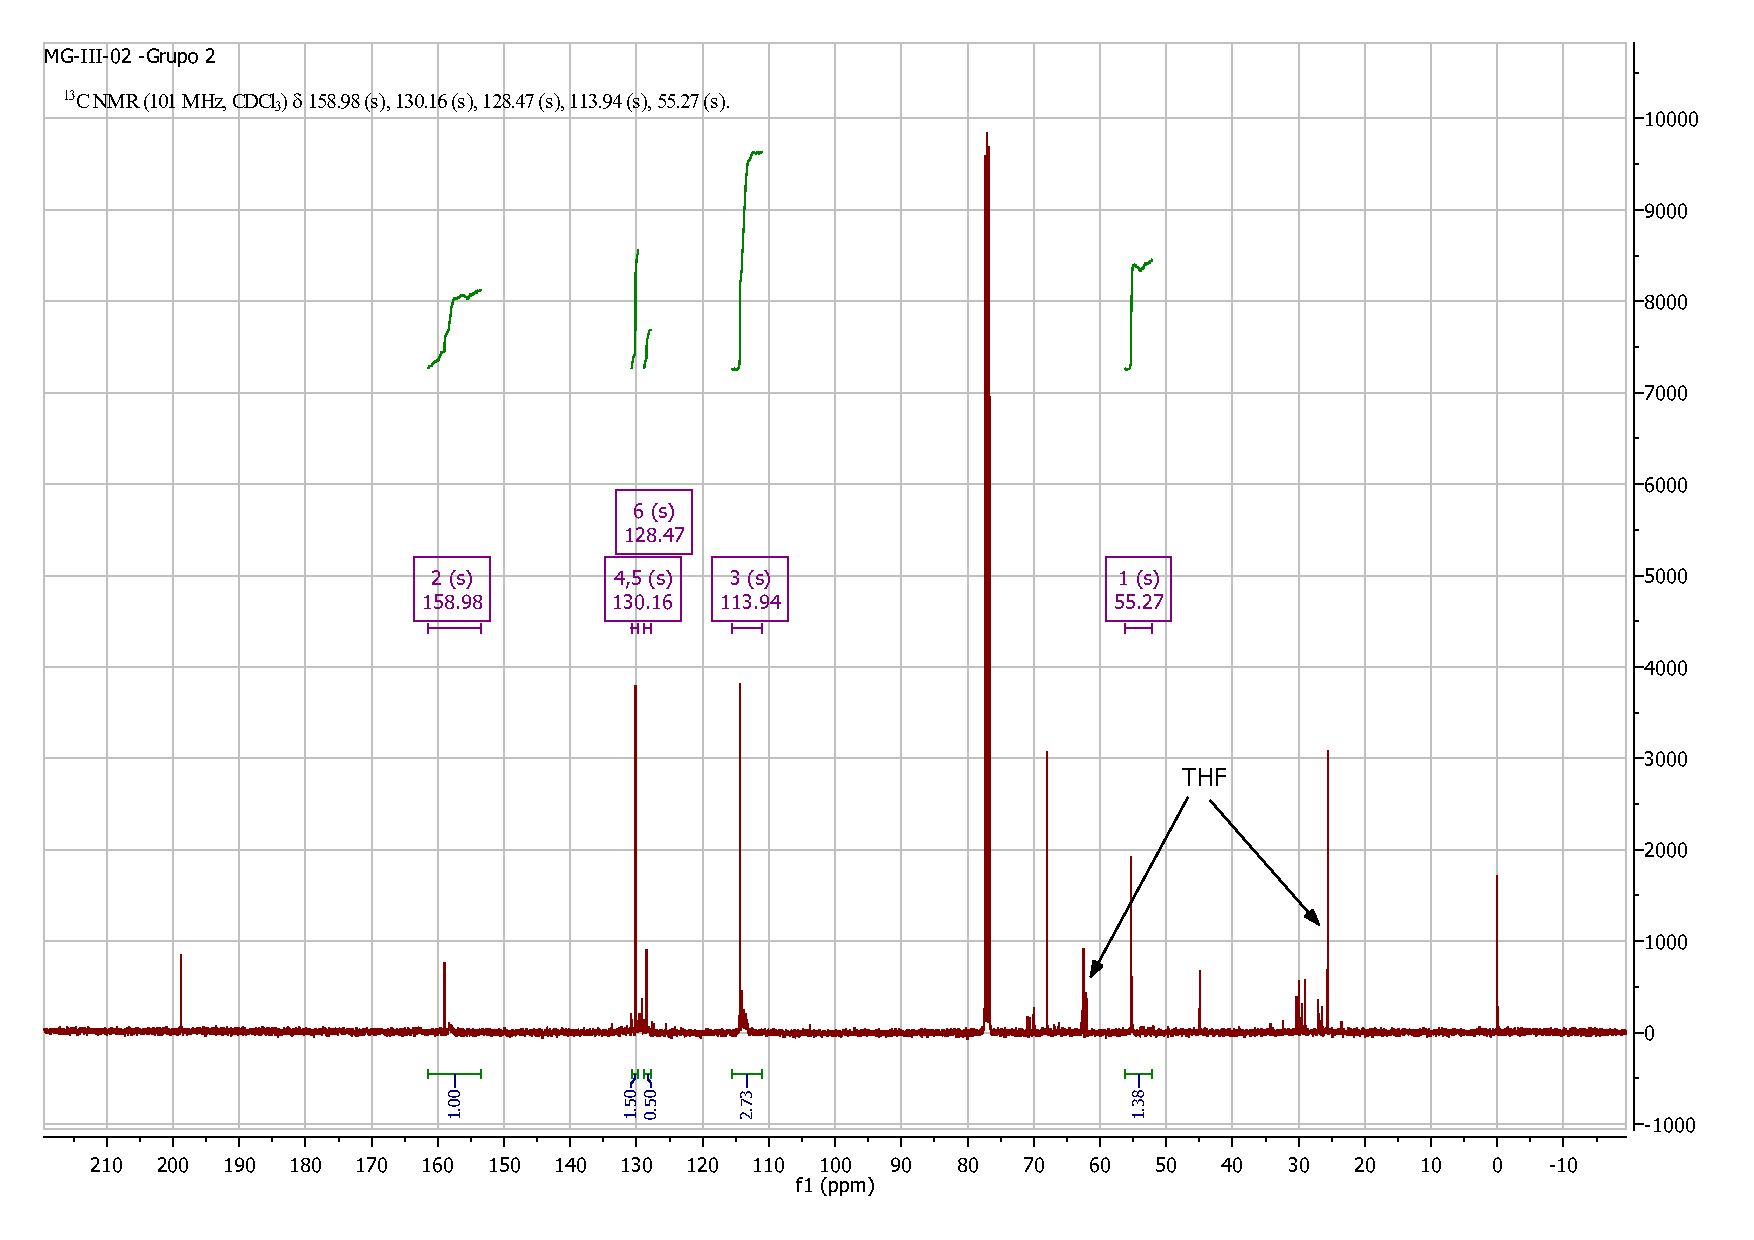
\includegraphics[height=0.7\textheight]{RMN/C.pdf}
		\captionof{figure}{$^{1}$HRMN del producto purificado.}
		\label{CHRM}
	\end{minipage}
}

\rotatebox{90}
{
	\begin{minipage}{\textheight}
		\centering
		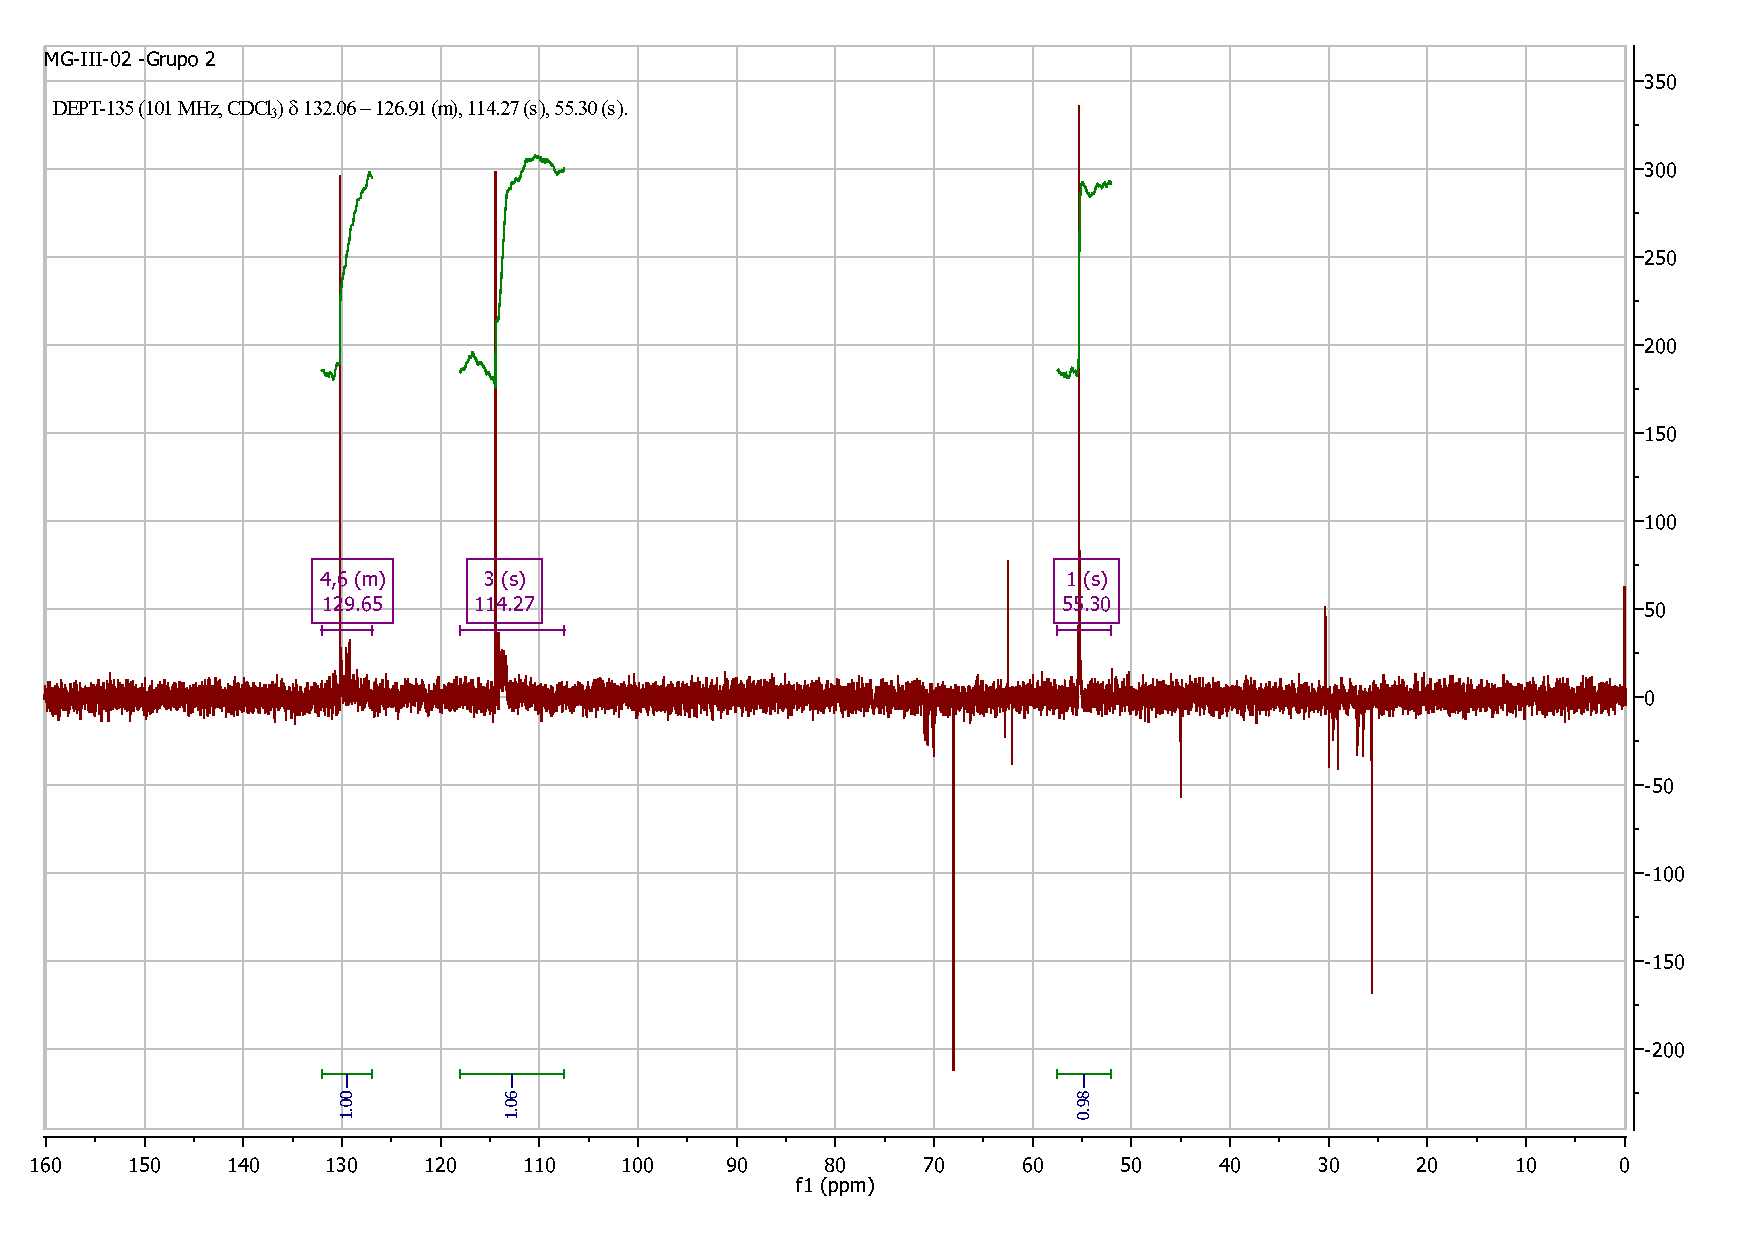
\includegraphics[height=0.7\textheight]{RMN/DEPT.pdf}
		\captionof{figure}{DEPT-135 del producto purificado.}
		\label{DEPT}
	\end{minipage}
}
\end{document}